\chapter{Subsystems}
\label{chap:subsystems}

In this chapter, the individual subsystems of the rover system will be discussed in more detail.

\section{Structure and Mechanisms}
\label{sec:mechanics}

The Structure and Mechanisms subsystem mainly deals with the accommodation of the payloads and all components that are necessary for the operation of the rover system. This also includes the mechanisms that are necessary for the rover system to ensure functionality 

\subsection{Storage Configuration and Rover Deployment}

The Main Characteristics of the Rover Chassis design of INSPIRE focuses on compact storage geometry and low Mass. 
During the design process it's been possible to achieve a reduce of volume in comparison to the first INSPIRE chassis design of about xxx~\%.
The geometry data in storage configuration is shown in figure %\autoref{fig:StaticAnalysis}.
The storage volume that is required is 131~l.
For the Rover Deployment there had been a lot of possible concepts, for example a sky crane, a robotic arm or a ramp. Depending of the reason that there are no further informations about the TRIPLE Lander and that the complexity of such a deployment system should be as simple as possible, the decision felt on a ramp where INSPIRE will drive slowly downwards the surface of Europa. 
A possible concept of the rover deployment is shown in the following figure %\autoref{fig:StaticAnalysis}.

\subsection{Exploration Configuration}

When the deployment is successfully done, INSPIRE has to switch from storage - to exploration configuration.
This will be possible with a cogwheel mechanism which will be operated by two Motors (QUELLENVERWEIS). When the wheel forks are horizontal to the ground, the rover is ready for its journey.
In order to maintain the rover stability while driving on rough terrain an averaging differential mechanism is needed.
This will be achieved by a planetary gear with a transmission ration of 1:1.
One bogie then will execute a counter movement du to the tilt of the other bogie.

\subsection{Static Analysis}

As part of the design process, it was necessary to perform a static analysis of the chassis. The following load cases were considered: \\
- Stowed configuration inside the TRIPLE lander on Europa \\
- Exploration configuration on the surface of Europa \\
The analysis was created with the computer aided design software "Autodesk Inventor". 
The results of this analysis are shown in the following \autoref{fig:StaticAnalysis}.

\begin{figure}[htb]
     \centering
     \begin{subfigure}[b]{0.49\textwidth}
         \centering
         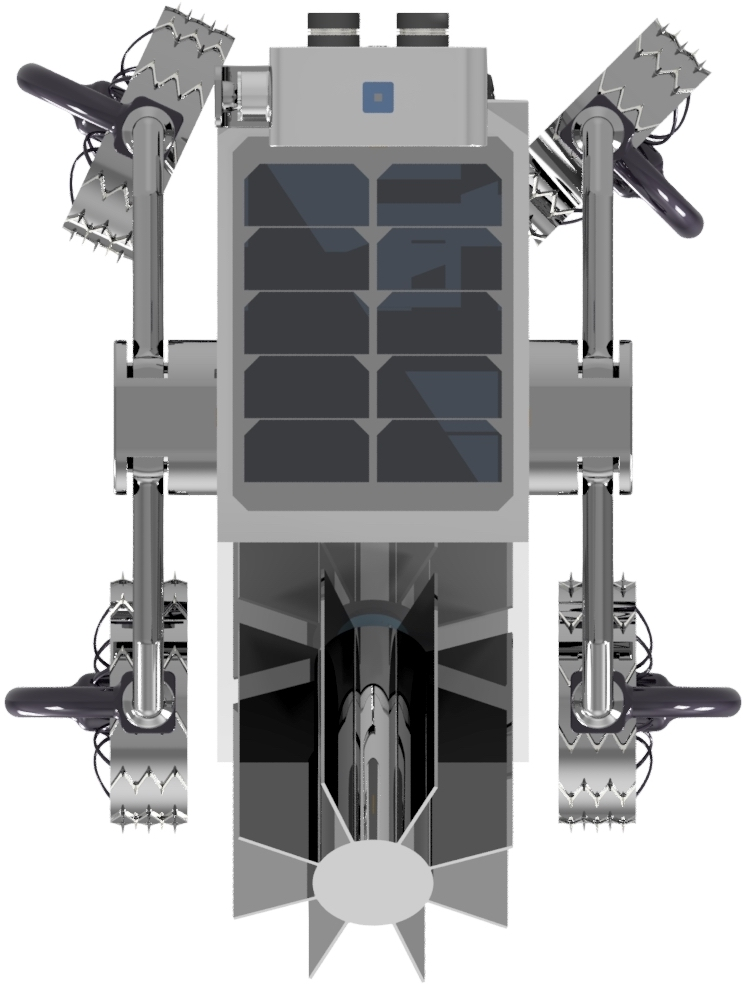
\includegraphics[width=\textwidth]{Media/INSPIRE_Locomotion}
         \label{fig:StoreConfig}
     \end{subfigure}
     \hfill
     \begin{subfigure}[b]{0.49\textwidth}
         \centering
         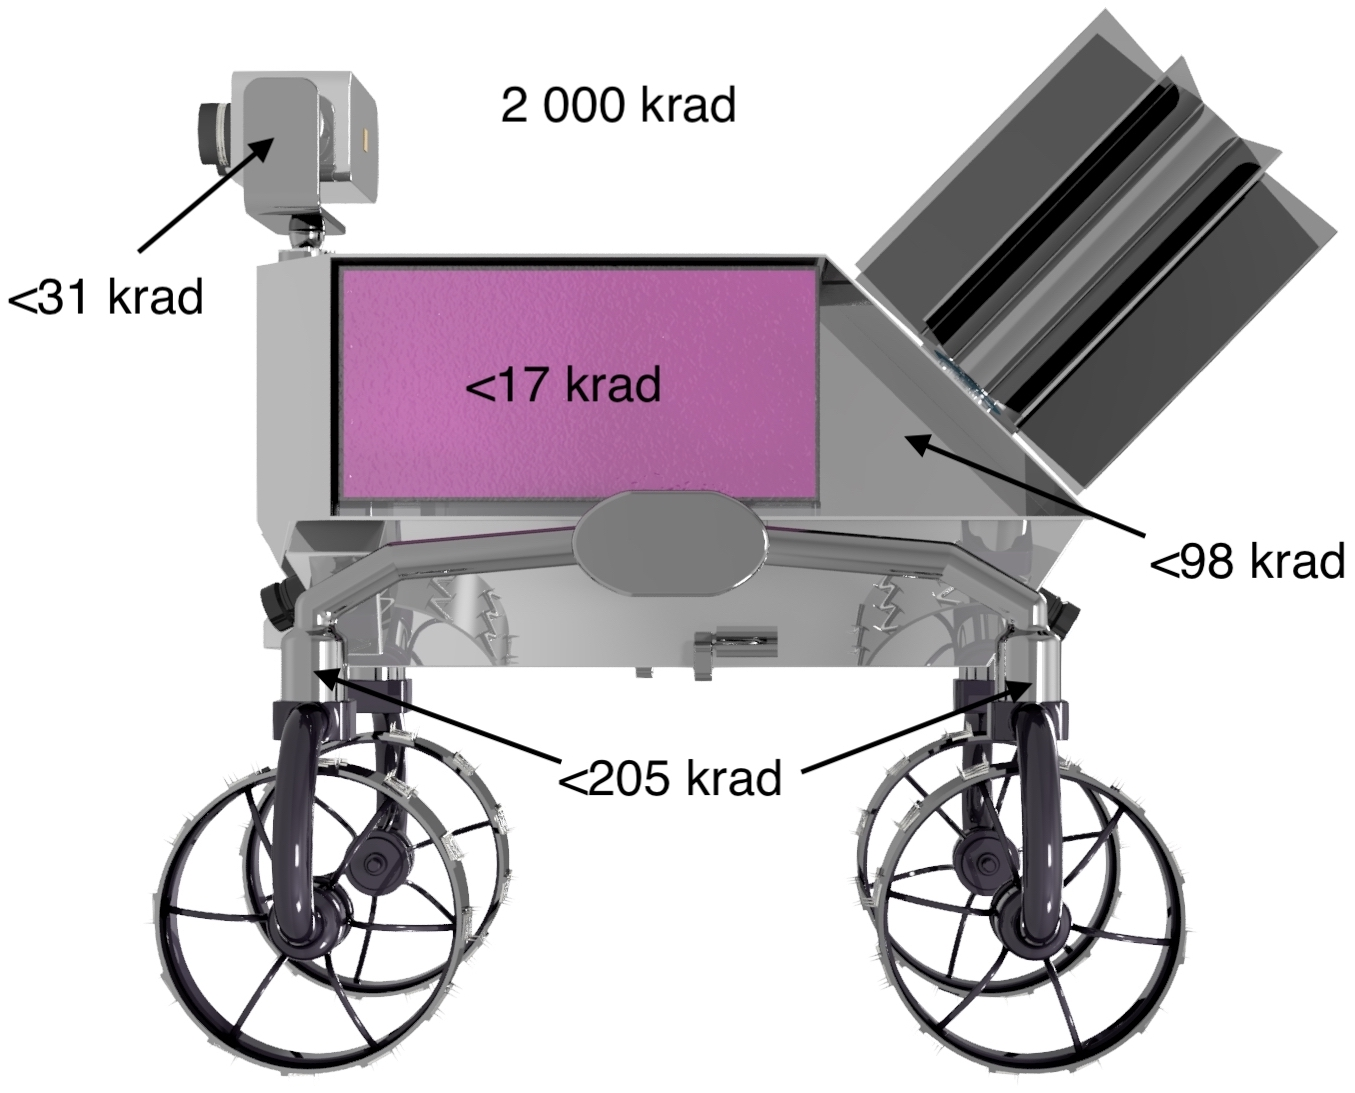
\includegraphics[width=\textwidth]{Media/INSPIRE_Radiation}
         \label{fig:ExplConfig}
     \end{subfigure}
     \hfill
     \caption{Results of the Static Analysis in Inventor. From left to right: Storage Configuration, Exploration Configuration }
     \label{fig:StaticAnalysis}
\end{figure}

\subsection{Mass Budget}

A really important part of each space system is the mass budget. Due to the strict mass restriction, it was quite difficult to find a suitable concept that is both light and space-saving. In order to make the design process of INSPIRE more effective, a specially selected preferred maximum mass of the chassis with the mechanisms of 5~kg was chosen which could also be adhered to. The following table lists the masses of the individual components of the structure and mechanisms system. 
A table with all components of the INSPIRE Rover system is shown in %\autoref{Muss noch verlinkt werden!}.

%-------------------------------------------------------------------------------
\section{Locomotion} \label{sec:locomotion}
%-------------------------------------------------------------------------------

The locomotion subsystem deals with the aspect of how the rover moves and the technical design, including the selection of components such as motors or gears. Before the components can be determined, however, it is necessary to consider certain parameters and design drivers. These will be introduced in the following, and the decisions or estimations concerning the rover will be presented.

\subsection{Design Drivers for Rover Classification}
\label{sec:DesignDriversLoco}

%Initial considerations in the design of a rover's locomotion system are the environmental and operational conditions expected for mission operations, as well as design factors. 
The fundamental rover design can be described by the wheel formula 4x4x4, based on a tradeoff, listed in \autoref{app:DigitalAppendix}. A more detailed design and the main criteria related to this are summarised in \autoref{tab:Design Drivers Rover Movement}.

\begin{table}[htb]
\centering
\caption{Fundamental rover design and the respective design drivers.}
% for the rover movement technique regarding the environmental conditions on Europa and operating conditions.
\label{tab:Design Drivers Rover Movement}
\resizebox{\textwidth}{!}{%
\begin{tabular}{|l|l|}
\hline
\rowcolor[HTML]{B3BBD1} 
\multicolumn{1}{|c|}{\cellcolor[HTML]{B3BBD1}Wheeled System}                                                                                                                     & \multicolumn{1}{c|}{\cellcolor[HTML]{B3BBD1}4-Wheels}                                                                                                \\ \hline
\begin{tabular}[c]{@{}l@{}}One of the most common types of platform\\ - high level of experience\\ - high TRL\end{tabular}                                                       & \begin{tabular}[c]{@{}l@{}}Compared to 2-wheels:\\ - stability  can be ensured \(\rightarrow\) important for drilling\\ - \(MMP\) decreases\end{tabular} \\ \hline
\begin{tabular}[c]{@{}l@{}}Compared to other systems:\\ - analysis quite straightforward\\ - simplification \(\rightarrow\) one of the most critical design drivers\end{tabular} & \begin{tabular}[c]{@{}l@{}}Compared to 6-wheels:\\ - less complex \(\rightarrow\) simplification\\ - mass can be reduced\end{tabular}                \\ \hline
\rowcolor[HTML]{B3BBD1} 
\multicolumn{1}{|c|}{\cellcolor[HTML]{B3BBD1}All-Wheel Drive}                                                                                                                    & \multicolumn{1}{c|}{\cellcolor[HTML]{B3BBD1}All-Wheel Actuation}                                                                                     \\ \hline
\begin{tabular}[c]{@{}l@{}}- traction can be increased\\ - increase of \(DP\) and the slope angle \(\theta\)\end{tabular}                                                        & - reduces the risk of slippage on ice                                                                                                                \\ \hline
\end{tabular}%
}
\end{table}

Furthermore, the normal force on Europa can be calculated to \( W \:  = \:	m_\text{total} \cdot g_\text{Europa} \:  = \: 39.45 ~ \text{N} \). Since each wheel is individually driven and controllable, the parameters in the following are designed for one wheel; the normal force per wheel is correspondingly \(W_\text{w} = 9.8625 ~ \text{N}\).

\subsection{System Parameters}
\label{sec:SystemParametersLoco}

Regarding techniques of rover movement, it is crucial to consider the local conditions in which the rover will be operating. The surface of Europa can be assumed to be mainly covered by ice. However, since there are also geysers that transport water to the surface, surface areas may be covered by snow. Though Europa's surface temperature does not exceed 130 K, rather icy, hard-packed snow can be assumed. For this study, a conservative design of the rover is considered, with soil parameters of snow in Sweden as well as heavy clay as a substitute for a hard ice surface; both are listed in \autoref{tab:SoilParam}. Furthermore, the parameters depend on the width and diameter of the wheels of the rover. Therefore, several sizes dependent on the respective weight were selected and a limit per wheel was set to 200 g, illustrated in \autoref{tab:Geometry}. This constraint results in 6 configurations considered for the Rover system design, listed in \autoref{tab:Configurations}. All necessary geometrical dimensions of the locomotion system are shown in \autoref{fig:Ackerman}.

\begin{table}[htb]
\centering
\caption{Configurations for rover classification respective to the wheel width \(b\text{w}\), wheel diameter \(d_\text{w}\) and weight per wheel \(m_\text{w}\).}
\begin{adjustbox}{max width=\textwidth}
\begin{tabular}{cccc|cccc}

	\toprule
		\multicolumn{1}{l}{Configuration} & \multicolumn{1}{c}{\(b_\text{w}\) /m} & \multicolumn{1}{c}{Diameter \(d_\text{w}\) /m} & \multicolumn{1}{c|}{Weight \(m_\text{w}\) /kg} &  \multicolumn{1}{l}{Configuration} & \multicolumn{1}{c}{\(b_\text{w}\) /m} & \multicolumn{1}{c}{Diameter \(d_\text{w}\) /m} & \multicolumn{1}{c}{Weight \(m_\text{w}\) /kg}  \\

	\midrule
		
		1	&	0.05	&	0.1		&	0.127		& 	4	&	0.05	&	0.125	&	0.154	\\
		2	&	0.06	&	0.1		&	0.153		&	5	&	0.05	&	0.125	&	0.185	\\
		3	&	0.07	&	0.1		&	0.178		& 	6	&	0.05	&	0.15	&	0.185	\\

	\bottomrule
	
\end{tabular}
\end{adjustbox}
\label{tab:Configurations}
\end{table}



\subsubsection*{Trafficability Configuration}
\label{sec:DP}

The ability of traffic depends on the soil parameters as well as on the geometric dimensions of the wheels. The sinking depth \(z\) for each wheel of the rover can be determined to:

\begin{equation}
	z \:  = \:	\left( \frac{3 W_\text{w} \cos \theta}{(3-n)(k_\text{c} + b_\text{w}k_\phi) \sqrt{d_\text{w}}} \right) ^{\frac{2}{2n+1}}	.
	\label{eq:Sinkage}
\end{equation}

As shown in \autoref{fig:Sinkage}, the sinking depth \(z\) depends not only on the geometric conditions and soil parameters but also on the slope angle \(\theta\). Therefore, \(z\) can be determined for both soils with respect to \(\theta\) as plotted in \autoref{fig:Sinkage}. However, it can be assumed that for the expected soil, the following applies: \( z_{\text{HeavyClay}} \leq z_{\text{Europa}} \leq z_{\text{Snow}} \).

\begin{figure}[htb]
     \centering
     \begin{subfigure}[b]{0.49\textwidth}
         \centering
         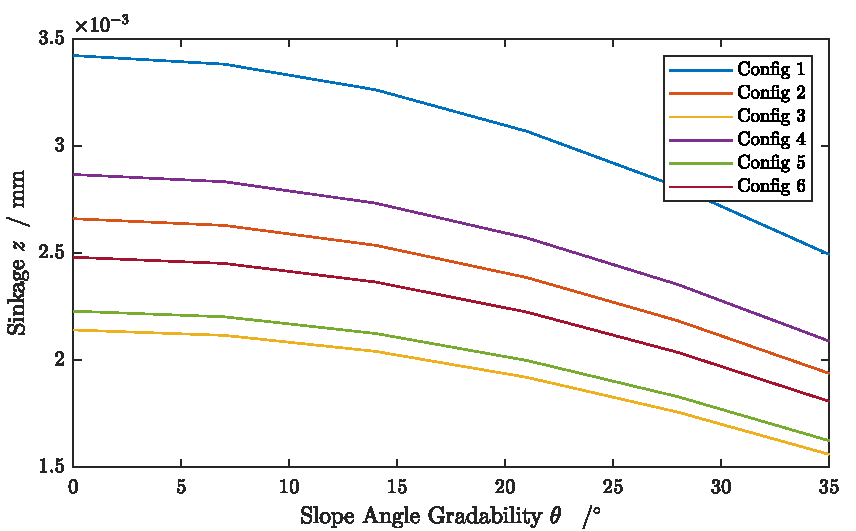
\includegraphics[width=\textwidth]{Media/Sinkage for each config in heavy clay.pdf}
         \caption{Heavy Clay}
     \end{subfigure}
     \hfill
     \begin{subfigure}[b]{0.49\textwidth}
         \centering
         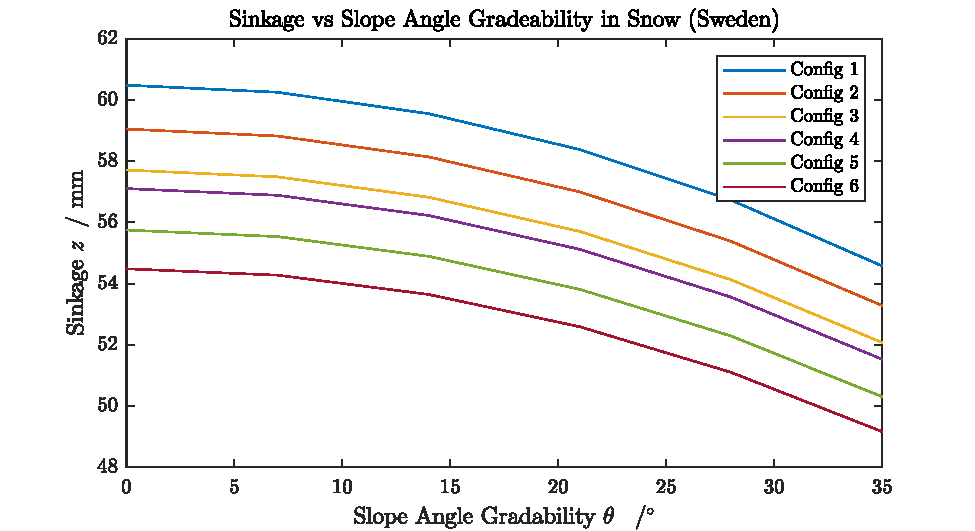
\includegraphics[width=\textwidth]{Media/Sinkage for each config in snow (Sweden).pdf}
         \caption{Snow (Sweden)}
     \end{subfigure}
     \caption{Wheel sinkage \(z\) as a function of the slope angle \(\theta\) of each configuration with different soil parameters, referred to \autoref{tab:SoilParam}.}
     \label{fig:Sinkage}
\end{figure}

The required power for the rover can be calculated by the resistances that have to be exceeded. For the total resistance, the following a applies:

\begin{equation}
 	R_{\text{total}} \:  = \: 
 	\underbrace{R_\text{compaction}}_{R_\text{c} = \: \frac{z^{n+1}}{n+1} \left( k_\text{c} + b  k_\phi \right)} + 
 	\underbrace{R_\text{rolling}}_{R_\text{r} = \: W_\text{w}  C_\text{rr}} +  
 	\underbrace{R_\text{gravity}}_{R_\text{g} = \: W_\text{w}  \sin \theta} +
 	\underbrace{R_\text{bulldozing}}_{R_\text{b} \rightarrow 0}. 	
 	\label{eq:Resistance}
 \end{equation} 

Due to the hard surface of Europa, it can be assumed that \( R_\text{b} \rightarrow 0\). In contrast to \( R_\text{g} \), \( R_\text{r}\) can be defined as constant. With a rolling resistance coefficient of \( C_\text{rr} = 0.02\), the resulting resistance is \( R_\text{r}\) = 0.1972~N \cite{rolling coefficient}. Analogous to \(z\), the lower limit of \(R_{\text{total}}\) with soil properties of heavy clay is plotted in \autoref{fig:RClay}, while the upper limit is shown in \autoref{fig:RSnow} for snow.

In addition to the resistance that needs to be exceeded in order to move, a maximum limit can also be determined. The ground thrust \(H\) indicates the amount of traction that can be achieved before the wheels slip.  Therefore, following applies:
\begin{equation}
	H \:  = \: A \cdot c + W_\text{w} \cdot \tan \Phi , 
	\label{eq:}
\end{equation}
 with the wheel ground contact area \(A = \frac{\pi}{4} \cdot b_\text{w} \cdot l_\text{w}\) and the ground contact length \(l_\text{w}=\frac{d_\text{w}}{2}\cos^{-1}\left(1 - \left( \frac{2z}{d_\text{w}} \right) \right)\). As a result, the absolute upper limit of traction is presented in \autoref{fig:HClay} for heavy clay and \autoref{fig:HSnow} for snow. 
 

\begin{figure}[htb]
     \centering
     \begin{subfigure}[b]{0.49\textwidth}
         \centering
         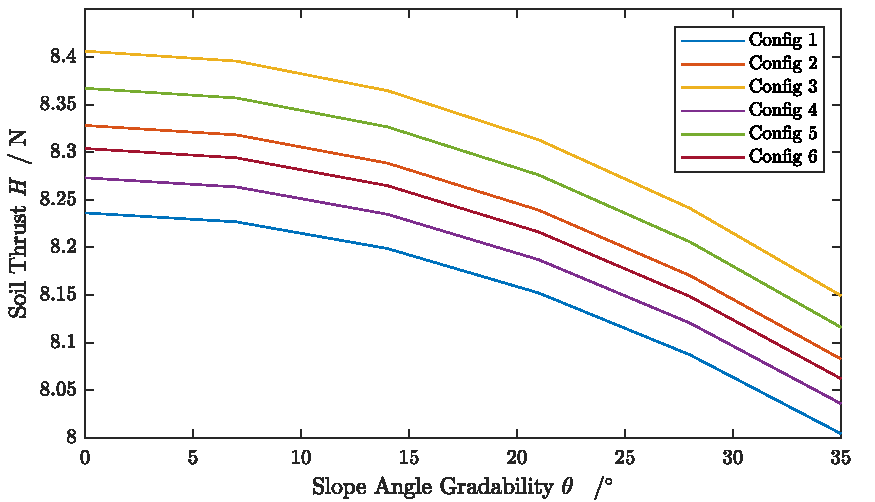
\includegraphics[width=\textwidth]{Media/Soil Thrust Heavy Clay.pdf}
         \caption{\(H\) for Heavy Clay}
         \label{fig:HClay}
     \end{subfigure}
     \hfill
     \begin{subfigure}[b]{0.49\textwidth}
         \centering
         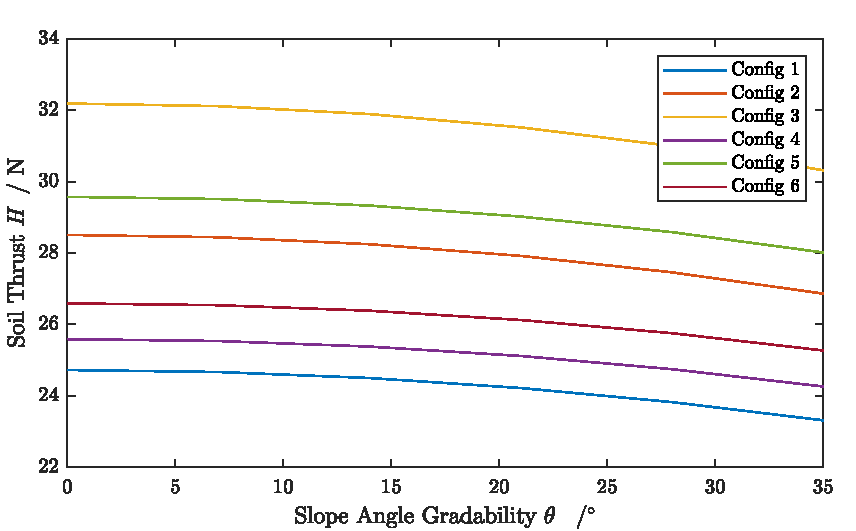
\includegraphics[width=\textwidth]{Media/Soil Thrust Snow.pdf}
         \caption{\(H\) for Snow (Sweden)}
         \label{fig:HSnow}
     \end{subfigure}
     \hfill
     \begin{subfigure}[b]{0.49\textwidth}
         \centering
         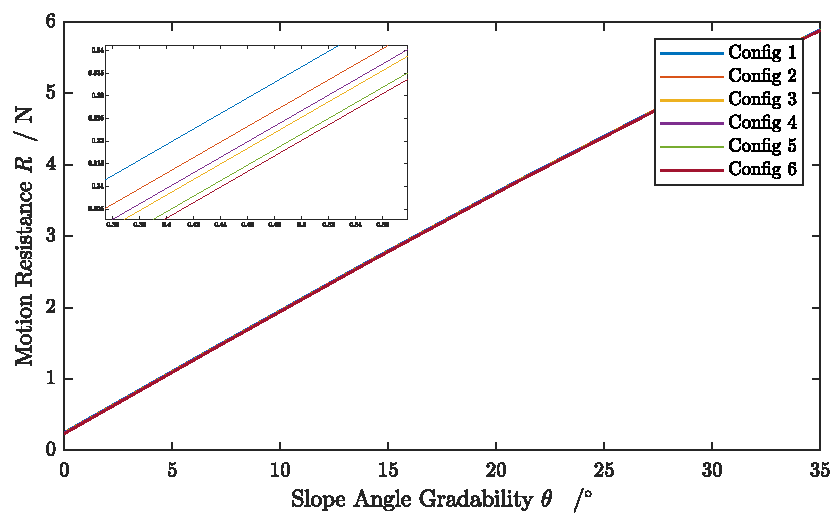
\includegraphics[width=\textwidth]{Media/ResistanceHeavyClay.pdf}
         \caption{\(R_\text{total}\) for Heavy Clay}
         \label{fig:RClay}
     \end{subfigure}
     \hfill
     \begin{subfigure}[b]{0.49\textwidth}
         \centering
         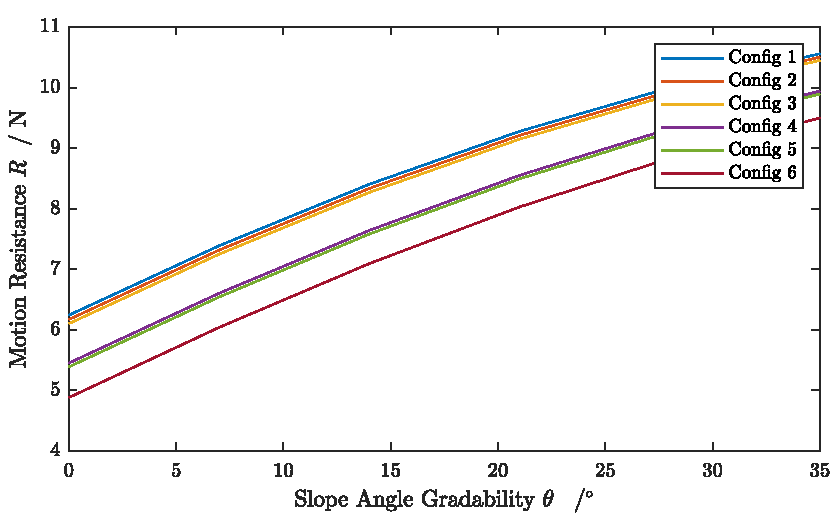
\includegraphics[width=\textwidth]{Media/ResistanceSnow.pdf}
         \caption{\(R_\text{total}\) for Snow (Sweden)}
         \label{fig:RSnow}
     \end{subfigure}
     \caption{Comparison of the rover's soil thrust versus the motion resistance to exceed, each for the soil parameters of snow in Sweden and heavy clay, referenced to \autoref{tab:SoilParam}.}
     \label{fig:SoilThrust_MotionResistance}
\end{figure}

In addition to the determined parameters, it should also be verified that the mean maximum pressure \(MMP\) does not increase excessively due to the selected geometric parameters \cite{MMP}. For this conservative calculation, a rigid wheel is assumed, whereby for the deflection \(\delta\) applies, that \( 0 \leq \delta \leq 0.1 d\). For terrestrial snow, 40~kPa should not be exceeded, but ideally the \(MMP\) should be less than 10~kPa \cite{Bekker}. The associated verification calculation can be found in \appref{app:MMP}. \\ 
For the rover design, configuration 6 is chosen as it offers the lowest resistance to exceed whilst maintaining the lowest \(MMP\). As shown in \autoref{fig:MMP}, the \(MMP_\text{Config6}\) is less than 10~kPa for \(\delta \geq 0.01\)~mm . It should be noted, that the rover has additional grousers. These are enhancing the traction, whereby the maximum reachable soil thrust \(H\) can be increased. However, the grousers are not taken into account in this study, as this is a conservative estimation, and the grousers can be seen as a further design improvement. 

\subsubsection*{Steering}
\label{sec:Steering}

Since the rover has an all-wheel actuation, it can be operated with on-point steering and, in order to avoid greater obstacles, with Ackerman steering. Considering that with Ackerman steering the radius of the outer wheels is at a greater distance in the circumventing circle than that of the inner wheels, the angles of the wheel positions, which are important for the control of the rover, are further examined in \appref{app:Ackerman}.



\subsubsection*{Hardware Selection}
\label{sec:HardwareLoco}

For the wheel driving system, BLDC motors were chosen. In contrast to stepper motors, these are optimised for a uniform torque and not for precise motion control. The resulting power of each wheel can be calculated with respect to the required torque \(\tau\) and the estimated velocity \(v\):

\begin{equation}
	P \:  = \:	\underbrace{\tau}_{= \:	R_\text{total} \left(\frac{d_\text{w}}{2} - \delta \right)} \left(\frac{2v}{d_\text{w}} \right).
	\label{eq:power}
\end{equation}

The motors are designed to produce the minimum achievable power for any soil condition and a slope angle of \(\theta_\text{max.} = 35^\circ\), listed in \autoref{tab:TorquePower} and velocities of \(0.1 \leq v \leq 1\)~m/s are achievable. However, as indicated in \autoref{fig:SoilThrust_MotionResistance}, higher power up to \(H\) can also be generated. Additional planetary gears increase the produced torque with a reduction ratio of 21:1 to \(\tau_\text{max} = 0.5\)~Nm. For the steering system, space grade stepper motors are selected, as a precise motion control is required. Additional information of the motors and gears can be found in \autoref{app:DigitalAppendix}.


\subsection{Deployment mechanism}

The deployment mechanism enables the rover to be stored in the lander in a space-saving arrangement. Two stepper motors are activated in the axle joints for this purpose. In addition, two further inactive motors are installed for redundancy. Stepper motors have the additional advantage that they maximise the holding torque. If in a further design step it should become apparent that the torque is not sufficient, a worm gear could be installed which has a self-retaining function. In addition to deploying after landing, the mechanism is used to reduce the distance to the ground for drilling. 


%-------------------------------------------------------------------------------
\section{Electrical Power System}
%-------------------------------------------------------------------------------
\label{sec:EPS}
The EPS (Electrical Power System) is the subsystem responsible for the electrical power supply of INSPIRE. It consists of four funadmental parts, which are the energy source, the PCDU unit (Power Control and Distribution) and the Energy Storage as well as the rover subsystems as the consumers. The EPS is visualized in \autoref{fig:epsflowchart}.

\begin{figure}[htb]
{\centering
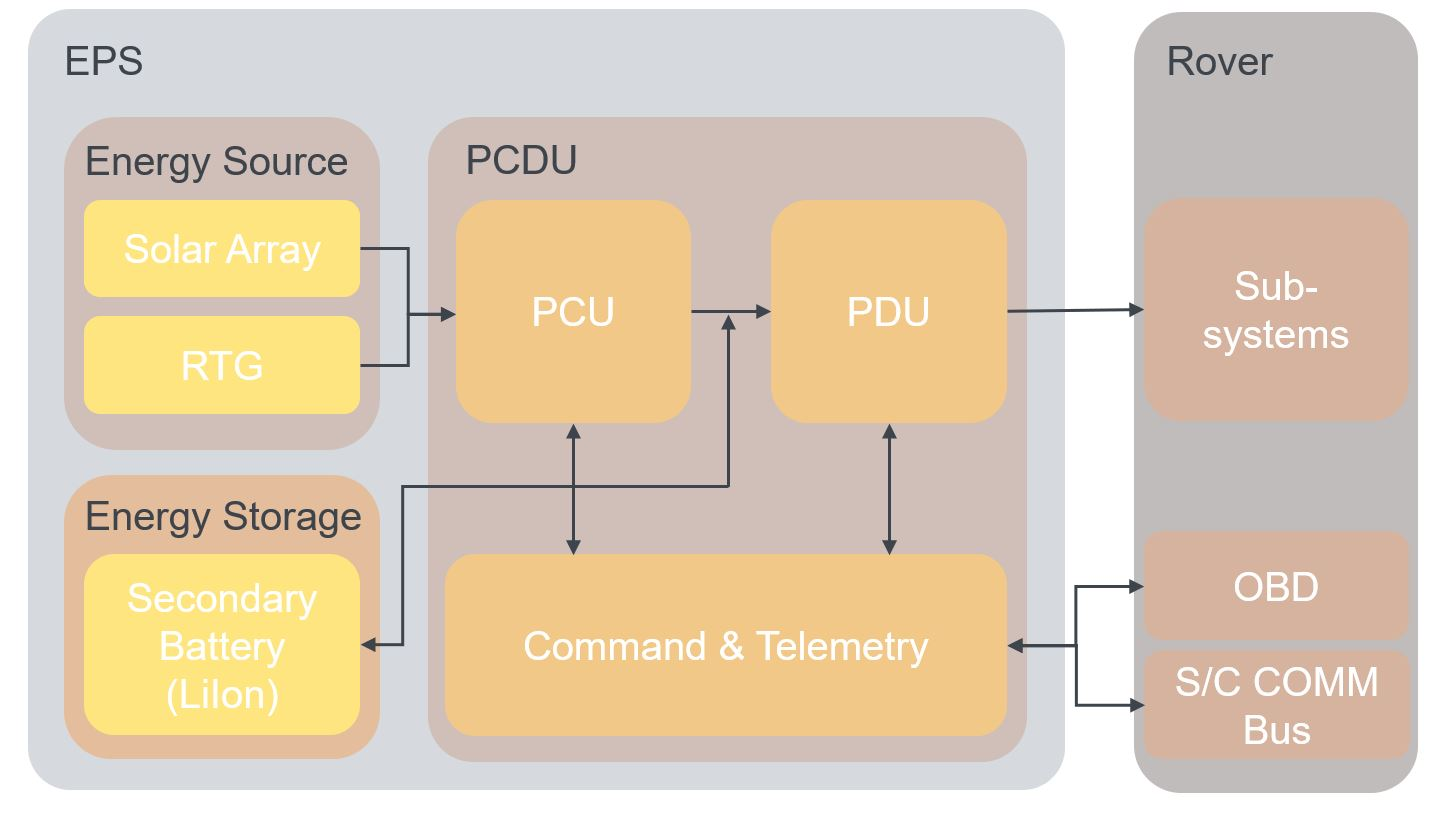
\includegraphics[width=0.7\textwidth]{Media/epsflowchart}
\caption{Functional Flow Chart Diagram for the EPS Subsystem.}
\label{fig:epsflowchart}
}
\end{figure}


\subsection{EPS Budget and Overview}
\autoref{fig:epspowersummary} summarizes the power budget of INSPIRE based on the rover system modes defined in \autoref{chap:rovsubmod}. The holistic power budget can be found in \autoref{tab:powerbudgetcomplete}.
As can be seen, the Locomotion mode has the highest demands on the EPS. The two payload modes also have a high power demand. The Communication mode also has a high consumption. However, since this is primarily used at night and the rover can be charged again afterwards without any problems, it does not place any major restrictions on the power budget. Idle/Perception mode has a low consumption, but is usually used for a long time at a stretch and therefore also places high demands on the EPS. In Charging mode, the EPS is able to charge $8.82 \ W_\text{el} $.


\begin{figure}[htb]
{\centering
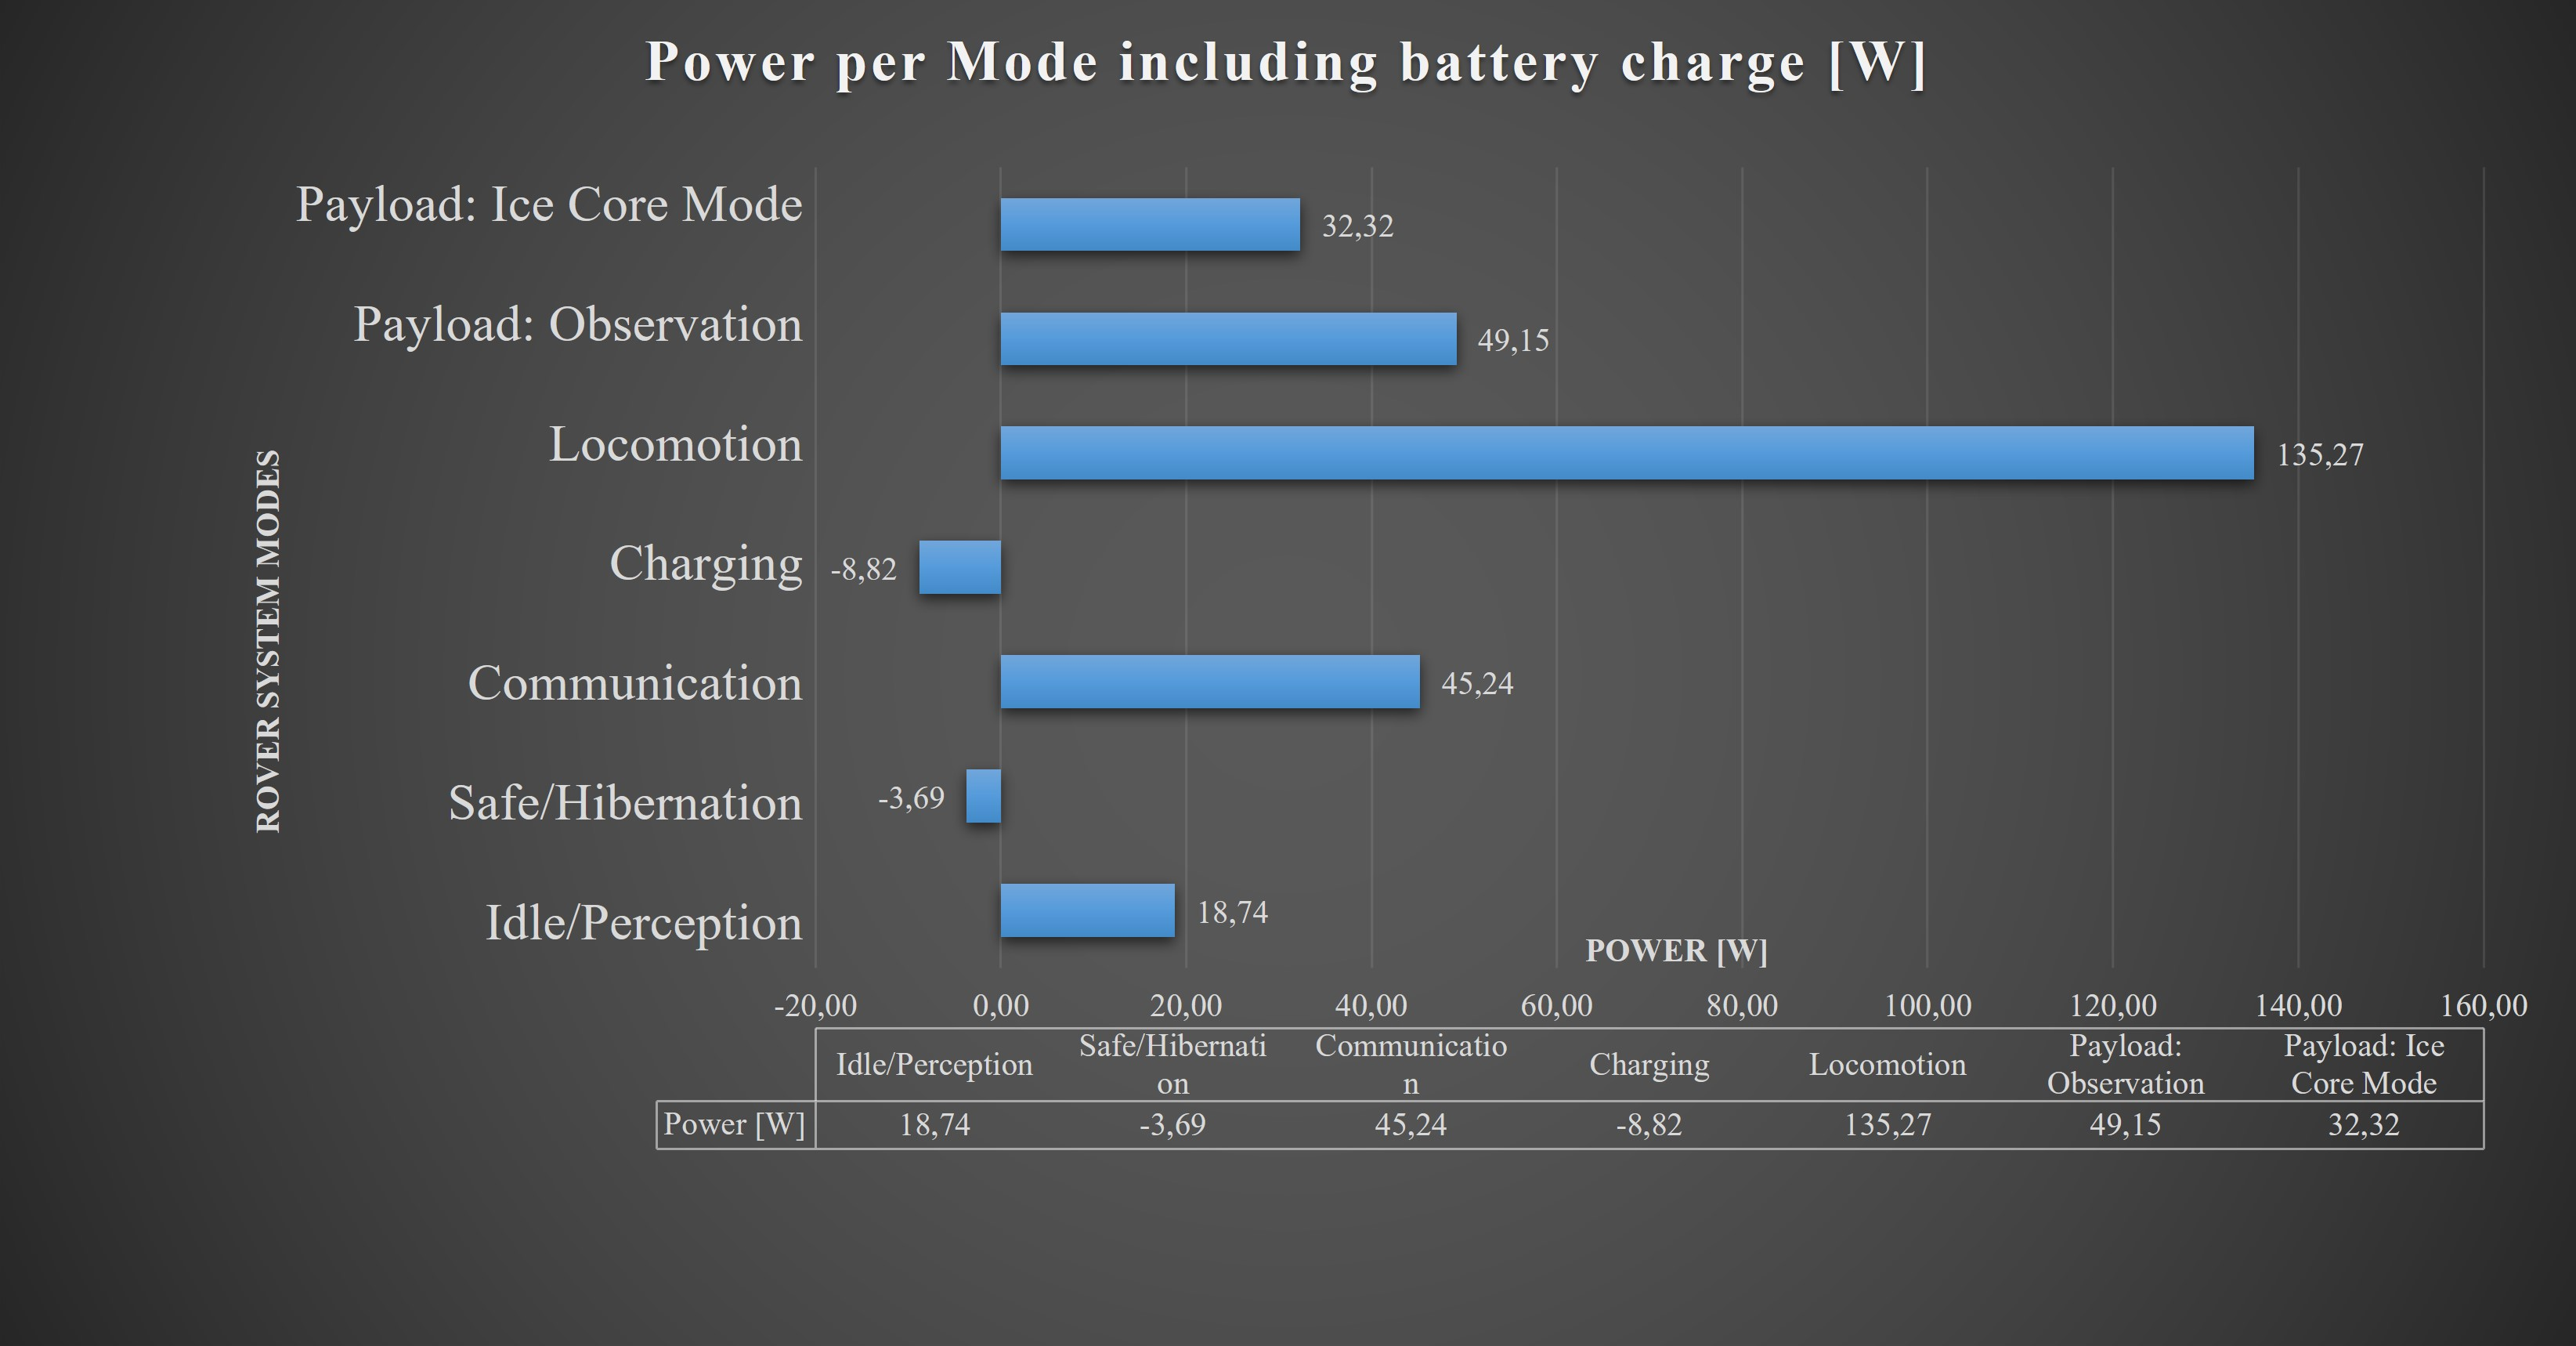
\includegraphics[width=0.7\textwidth]{Media/epspowersummary}
\caption{Functional Flow Chart Diagram for the EPS Subsystem.}
\label{fig:epspowersummary}
}
\end{figure}


%\begin{table}[htb]
%\centering
%\begin{tabular}{|c|c|}
%\hline
%\textbf{Rover System Mode} & \textbf{\begin{tabular}[c]{@{}c@{}}Total Rover \\ Power Demand \\ including battery charge $P_\text{mode}$ [$W_{el}$]\end{tabular}} \\ \hline
%Idle/Perception            & $15.25$                                                                                                                             \\ \hline
%Safe/Hibernation           & $-5.84$                                                                                                                             \\ \hline
%Communication              & $36.92$                                                                                                                             \\ \hline
%Charging                   & $-7.04$                                                                                                                             \\ \hline
%Locomotion                 & $232.36$                                                                                                                            \\ \hline
%Payload: Observation       & $15.41$                                                                                                                             \\ \hline
%Payload: Ice Core Mode     & $9.77$                                                                                                                              \\ \hline
%\end{tabular}
%\caption{Overview of the Power Budget of INSPIRE.}
%\label{tab:powbud}
%\end{table}


\subsection{Energy Source}
For the energy generation of INSPIRE many possible sources were taken into consideration for a trade-off. As a conclusion of this trade-off the decision was made to utilise a Radioisotope Thermoelectric Generator (RTG) as the main energy source for INSPIRE.\\
As the research couldn't find an RTG with a mass suitable for INSPIRE, the solution was to scale down a bigger RTG as an approximation. As a baseline of the scaling the eMMRTG (Enhanced Multi Mission Radioisotope Thermoelectric Generator) was utilised, which is currently under development at NASA and is especially designed for deep space missions like Europa. For the scaling a goal RTG mass of $m_\text{RTG}=3~\text{kg}$ was defined and the eMMRTG was scaled down using the given data.\\
In \autoref{tab:esmmrtg} the scaling results for the eSMMRTG (Enhanced and Scaled Multi Mission Radioisotope Thermoelectric Generator) are listed. The eSMMRTG has a BOL specific power of $\alpha_\text{BOL}= 4.0 \ \frac{\text{W}_\text{el}}{\text{kg}}$ and provides an electrical power of $P_\text{el} = 12.08~\text{W}_\text{el}$ during the mission duration\cite{R.Abelsonetal..2004}\cite{S.Magdum.2019}\cite{Holgate.2015}\cite{eMMRTG.NASA}\cite{Lakdawalla.2018}.



%The outcome of this trade-off is shown in \autoref{fig:epssourcetradeoff} for the most promising energy sources. 

%
%\begin{figure}[htb]
%{\centering
%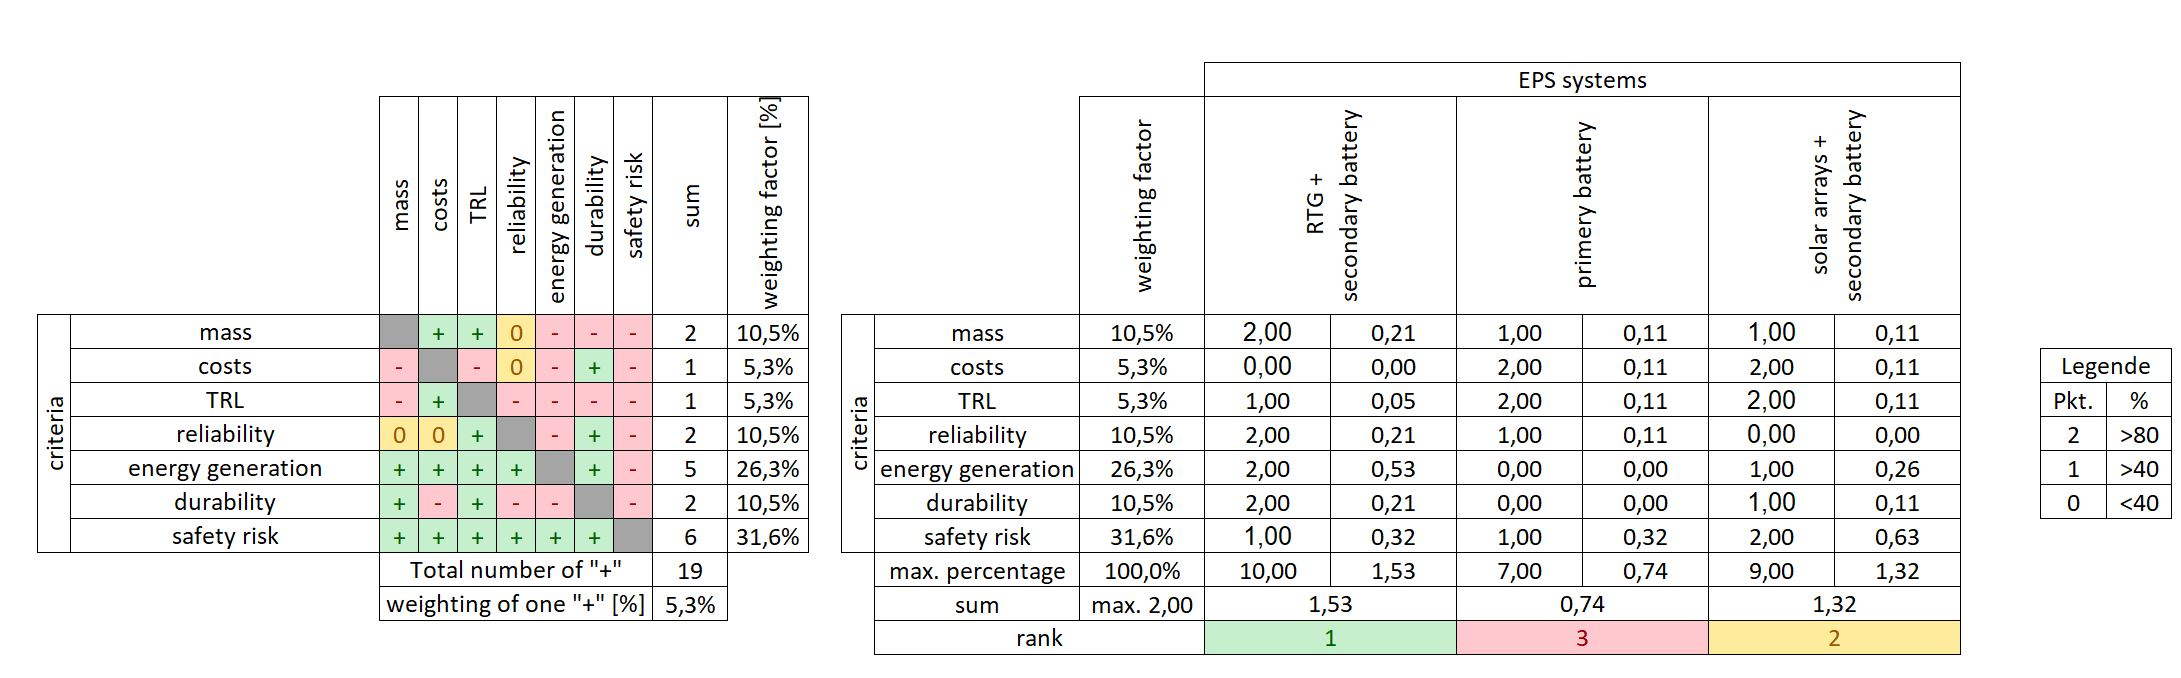
\includegraphics[width=0.7\textwidth]{Media/epssourcetradeoff}
%\caption{Trade-Off Conclusion for the EPS Energy Source.}
%\label{fig:epssourcetradeoff}
%}
%\end{figure}

\begin{table}[H]
\centering
\caption{Parameters for the scaled eSMMRTG based on the eMMRTG.}
\begin{tabular}{lcc}
\toprule
Scaled eSMMRTG Parameter &	Unit	&   Value            \\
\midrule
\textbf{System Mass} $m_\text{RTG}$ & kg  & \textbf{3.5}     \\
BOL Specific Power $\alpha_\text{BOL}$ & $\frac{W_{el}}{\text{kg}}$  & $4.0$     \\
BOL Power $P_{\text{el},\text{BOL}}$ & $ W_{el}$                    & $14$       \\
Isotrop                 &         -                           & Pu-238   \\
Isotrop Half-Life & a                                       & $87.7$     \\
Flight time and Storage (incl. Margins) & a                & $7$        \\
Power Loss Degradation until BOM & $\ W_{el}$                 & $0.56$     \\
BOM Power $P_{\text{el},\text{BOM}}$ & $\ W_{el}$                    & $13.44$    \\
Europa Day Duration & h                                     & $85$       \\
Mission Duration & d                                        & $106.25$   \\
End of Mission Power $P_{\text{el},\text{EOM}}$ & $\ W_{el}$         & $13.42$   \\
\textbf{Final Power for Study} $P_\text{el}$ (incl. $10~\%$ scaling Margin) & $\ W_{el}$  & \textbf{12.08}    \\
\bottomrule
\end{tabular}
\label{tab:esmmrtg}
\end{table}

Furthermore INSPIRE will also be equipped with some radiation hardend solar arrays as already explained in \autoref{subsec:radhard}\cite{FraunhoferInstituteforSolarEnergySystemsISE.2021}. Since these solar cells are primarily used for technology testing, the mission must also be able to operate completely without this generated energy. For this reason, and because the expected energy generated by the solar cells is minimal, only the energy generated by the RTG is considered for the Phase 0 Study. However, it should be noted that these solar cells will also generate a certain amount of energy, which will benefitial for the EPS.


\subsection{Energy Storage} 
For the energy storage of INSPIRE many possible battery types were taken into consideration for a trade-off. As a conclusion of this trad-off the decision was made to utilize LiIon batteries as the secondary batteries of INSPIRE. This decision is primarly based on LiIon batteries high energy density, temperature range, robust performance and long operating and cycle life in extreme environments\cite{IRSatUniversityofStuttgart.2020}\\
As the RTG only generates a small constant power the main energy source during the mission will be the accumulated energy of the batteries. The rover will charge the batteries at night, so the next exploration day can start with full capacity. Furthermore the batteries have to be charged during day time to maintain operations.\\
For the sizing of the batteries, the rover motion was chosen as the design driver, since this is the highest energy consuming state of the rover and additionally mission critical for INSPIRE. The rover motion consists of an interaction of the Locomotion and Perception mode as already mentioned in \autoref{chap:Operation}. Therefore it was defined that INSPIRE shall be able to drive $ 50$ m (including alternating Locomotion and Perception Mode) with a fully charged Battery. Furthermore the battery mass shall not exceed $2$ kg. The required battery capacity $C_\text{Batt,req}$ can be caculated using \autoref{eq:batreq}. The results are listed in \autoref{tab:batsize} \cite{S.Klinkner.2021}.


\begin{equation}
C_\text{Batt,req} = \frac{P_\text{el,req} \cdot t_e }{DoD \cdot \eta_\text{LiIon}}
\label{eq:batreq}
\end{equation}

\begin{table}[htb]
\centering
\caption{Power consumption mode used as design case for the battery sizing.}
\begin{tabular}{lccc}
\toprule
\textbf{Power Consumption Mode:}             &     \textbf{Unit}      & \textbf{Locomotion} & \textbf{Perception} \\
\midrule
Required Electrical Power $P_\text{el,req}$ & $\text{W}_\text{el}$         & $135.27$              & $18.74$               \\
Duration of the mode $t_\text{e}$ & s                         & $500$              & $15000$            \\
$DOD$ for Dimensioning               &     -          & $0.90$                & $0.90$                \\
Efficiency of LiIon Cells $\eta_\text{LiIon}$   &  -  & $0.95$                & $0.95$                \\
Required Battery Capacity per mode $C_\text{mode}$ & Wh & $21.97$              & $91.33$              \\
\textbf{Total Required Battery Capacity} $C_\text{Batt,req}$  & Wh & \multicolumn{2}{c}{\textbf{113.30}}               \\
\bottomrule
\end{tabular}


\label{tab:batsize}
\end{table}

Using these values a suitable battery cell and battery design configuration were conducted. Under consideration of these parameters the battery capacity $C_\text{Batt}$ can be calcuated:

\begin{equation}
C_\text{Batt} = C_\text{cell} \cdot V_\text{cell} \cdot N \cdot M .
\label{eq:batuse}
\end{equation}

According to the ECSS reliability restrictions 1 battery string must be substracted for dimensionsing. Furthermore a $30~\%$ margin on the energy content was applied. This leads to a final battery configuration with a capacity of $C_\text{Batt}=156.24$ Wh and a mass of $m_\text{Batt} = 1980$ g. The final battery values are listed in \autoref{tab:battery} \cite{SAFTBatteries.2018}.


\subsection{EPS Power Control and Distribution}
In order to ensure the full functionality of the EPS, the last main component to be selected is a suitable PCDU. As described in \autoref{fig:epsflowchart}, the PCDU forms the heart of the EPS and is an important interface to the OBC and COMM. Furthermore the PCDU shall be able to monitor and control the rover system if necessary through watchdogs, HPC (High Priority Commands) and direct connections to the OBC and COMM.\\
The PCDU has the challenging task not only to process the RTG as the main energy source, but also to process solar cells as secondary energy sources. Therefore, a PCDU was sought which has the required size, dimensions and range of functions. The research resulted in the Nova PCDU from Bradford DSI. In addition, margins were added to the PCDU to ensure feasibility\cite{BradfordSpace.2019}.

\section{Communications and Command \& Data-Handling}
\label{sec:comm}
The Communications subsystem consists of redundant transmitters and receivers which are cross strapped to four antennas and the OBC. Additionally hard wired connections linking the communication system to the PCDU enable for reboots via direct commands.\\
C\&DH is responsible for the generation of telemetry from the housekeeping boards and the execution of telecommands, as well as the storing and compressing of payload data. 

\subsection{Operational Concept}

Due to power and time constraints, the rover will transmit only telemetry during the locomotion and payload campaigns. Payload data will be compressed, stored and forwarded to the Lander at the end of a mission day. \\ 
 
To achieve the scientific output from \autoref{chap:sc-output} the transmission time per european day is calculated in \autoref{app:MissionDataOutput} (\autoref{tab:Tx-tptal}) and adds up to 38,23 minutes. 
	
\subsection{Communication System}
Requiring too many resources a direct link to earth has been deemed impractical. Instead communication for the INSPIRE mission is proposed to rely on a link between the rover and the Europa Lander. The lander then forwards data to earth via a satellite relay carrier which orbits the moon. The lander offers a 25 dB high gain antenna [Missing Reference] and a low gain antenna which is not further specified in literature.\\

The downlink from the rover to the lander has been identified as the critical transmission path. However, link budget considerations in \autoref{app:LinkBudget} reveal that a transmission to the LGA of the Europa Lander produces a link margin of $10,59~\text{dB}$, resulting in a Bit Error Rate of less than $10^{-4}$. The link budget has been performed under the conservative considerations listed in \autoref{tab:lb-param}.\\

Using the Landers LGA greatly increases robustness due to the elimination of pointing errors and higher margin for rover positioning error. Additionally, the INSPIRE rover’s communication link would not interfere with the Landers communication to the relay carrier by blocking the HGA.

\subsubsection{Component Selection}

Due to the considerably high link margin the focus is on low mass and low power components with flight heritage such as flown on CubeSat missions. Criteria with relatively small impact on the link budget such as component noise or even FEC have not been taken into account. The rover communication uses X-Band for increased compatibility with the lander and has a total system mass of less than $1~\text{kg}$. \\
Since radiation hardness was not included in most data sheets a total dose of $<20~\text{krad}$ was assumed in accordance with values for LEO [Missing Reference]. \\

The selected components are listed in \autoref{tab:ComCompComp}. 

\begin{table}[h]
\centering
\caption{Key criteria of selected communication components}
\begin{tabular}{lll|ll|ll}
\toprule
Component   & Supplier  & Part Description     & 1. Criteria   & Value    & 2. Criteria & Value          \\
\midrule
Transmitter & Sputnix   & SXC-XTX-01           & mass          & 0,195 kg & data rate   & 10 Mbit/s \\
Receiver    & Endurosat & S-Band receiver      & power         & max. 2 W & mass        & 0,220 kg       \\
Antenna     & Endurosat & patch antenna & mass          & 2,2 g    & frequency   & X-Band         \\
\bottomrule
\end{tabular}
\label{tab:ComCompComp}
\end{table}

Expected transmission times per mission day are less than 40 minutes (see \autoref{app:MissionDataOutput}, \autoref{tab:Tx-tptal}). Therefore the transmitter mass is identified as more critical than power. \\
Receiver duty cycles on the other hand range close to 100 \% (REFERENCE POWER BUDGET). Thus power has been identified as the most crucial criteria. \\
A passive X-Band antenna was selected due to compact dimensions and zero power consumption.  \\
The entire trade off can be found in (APP Trade off).

 \subsection{Command \& Data Handling}
 
 With respect to restricted power supply a redundant OBC hot-cold configuration stands to reason. Additionally, the standby mode is suggested during hibernation and charging modes relying solely on the PCDU (see chapter [Missing Reference]). 
Emphasis for the Electronics selection is placed on flight proven radiation hardness to increase mission robustness in the high radiation environment of the Jupiter system. 
Criteria of less importance are CPU speed and dimensions. \\

Instead of designing a new OBC board a trade-off was performed among existing single board computers. SBCs provide peripheral services such as bus interfaces, timer and memory in a flight proven configuration, which promises an effective mission development. \\

BAE Systems provides a SBC with their flight proven Power PC750 Architecture which withstands a total radiation dose of up to $1~\text{Mrad}$. The robustness comes at the cost of a $182~\text{MHz}$ processor speed (DATASHEET REFEreNCE). \\

Additionally a custom housekeeping board will be tasked with providing engine control peripherals and sensor read out electronics. 

%-------------------------------------------------------------------------------
\section{Thermal Control System} \label{sec:thermalcontrol}
%-------------------------------------------------------------------------------
The main object of the Thermal Control System (TCS) is to keep the electric components within their temperature limits, listed in \autoref{tab:tcs_limits}.
As a result of Europas low surface temperature, a small solar constant and the thin atmosphere the heat loss of the rover has to be minimised  \cite{Europa}.

\subsection{Concepts}
The main heat source of the rover is the waste heat of the RTG (see \autoref{sec:EPS}), which will be led by thermal straps to the temperature sensitive components.
Carbon-based straps \textit{LyNX}\textsuperscript{\tiny\textregistered} with a high thermal conductivity to density ratio will be used, \cite{ref_tcs_01}.
However, the thermal conductivity is highly dependent on the material temperature, see \autoref{fig:tcs_strap01}.
The curve was approximated by  a cubic  interpolation, \autoref{fig:tcs_lynx} and \autoref{eq:tcs_lynx}.
To consider heat loss as a result of surface contact and radiation, the thermal conductivity was reduced about 20\%.
%
\begin{figure}[h]
	\centering
	\subfloat[Temperature dependent thermal conductivity/density of \textit{LyNX}\textsuperscript{\tiny\textregistered} (yellow curve), copper, and aluminum, \cite{ref_tcs_01}.]{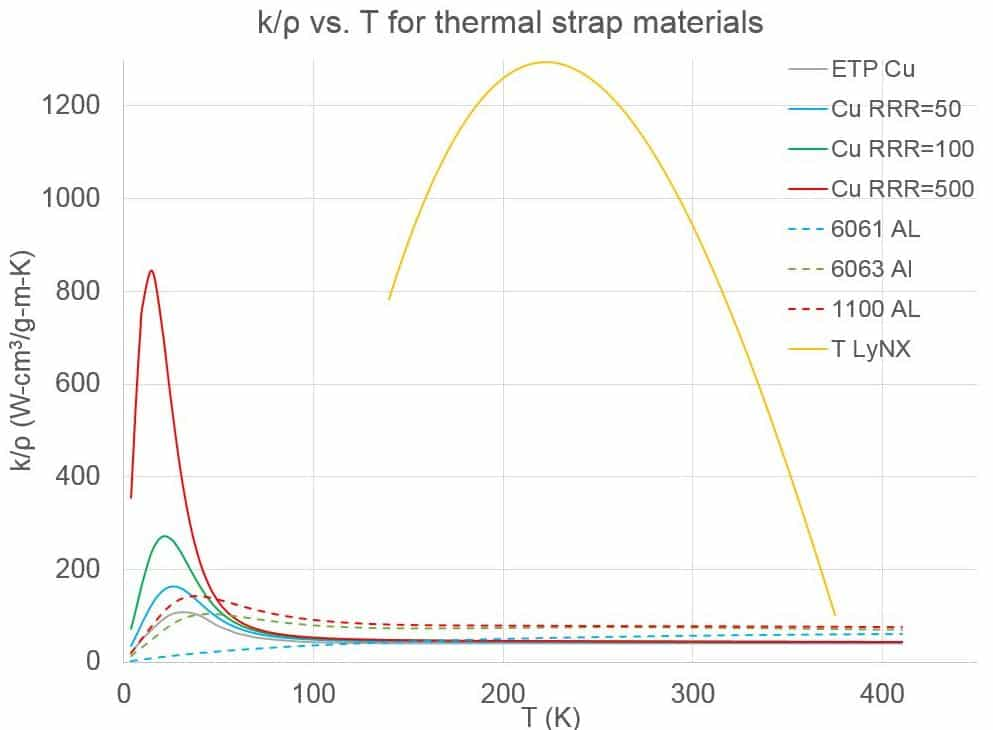
\includegraphics[height=0.3\textwidth]{Media/tcs_strap_01.JPG}\label{fig:tcs_strap11}}\qquad\qquad
	\subfloat[Example of a thermal strap, \cite{ref_tcs_01}.]{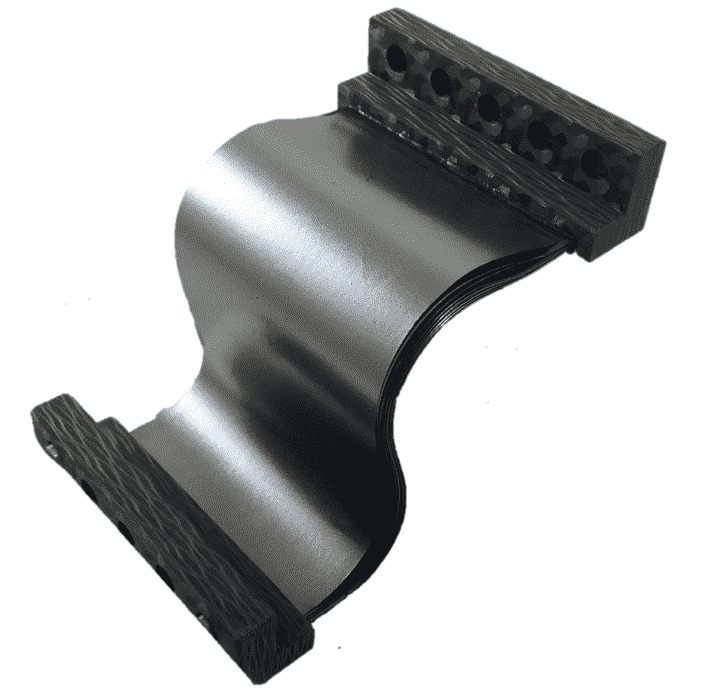
\includegraphics[height=0.2\textwidth]{Media/tcs_strap_02.png}\label{fig:tcs_strap12}}
	\caption{Carbon-based thermal strap \textit{LyNX}\textsuperscript{\tiny\textregistered}.}
	\label{fig:tcs_strap01}
\end{figure}
%
The camera, exposed on a mast, will be heated by a seperate, lightweight Radioisotope Heater Unit (RHU), which has  been used during several NASA missions \cite{ref_tcs_02}.
For the insulation, the material \textit{Aerogel} will be applied, which has a very low heat conductivity, \cite{ref_tcs_03}.

To avoid the risk of overheating, concerning the ebay, camera and drive engine, passive bi-metallic heat switches  will be  placed between the application and the connection interface (see \autoref{fig:tcs_switch01}).
These switches change their heat conductivity beyond a certain temperature due to the expansion of the disk (see \autoref{fig:tcs_switch21}).
It was assumed that the toggle temperature can be adapted by modifying the disk height.
The influence of the changed disk stiffness on the contact pressure and therefore the heat conductivity was neglected for this study.
The measured heat conductivity characteristic was divided in three linear sections (\autoref{fig:tcs_switch22}), to enable a simple modelling in the thermal calculation.
For most components, a cost-efficient sand blasting of the surface is applicable.
For special requirements, white paint will be used, \autoref{tab:tcs_surf}.

\begin{figure}[H]
	\centering
	\subfloat[Closed switch, high heat conduction.]{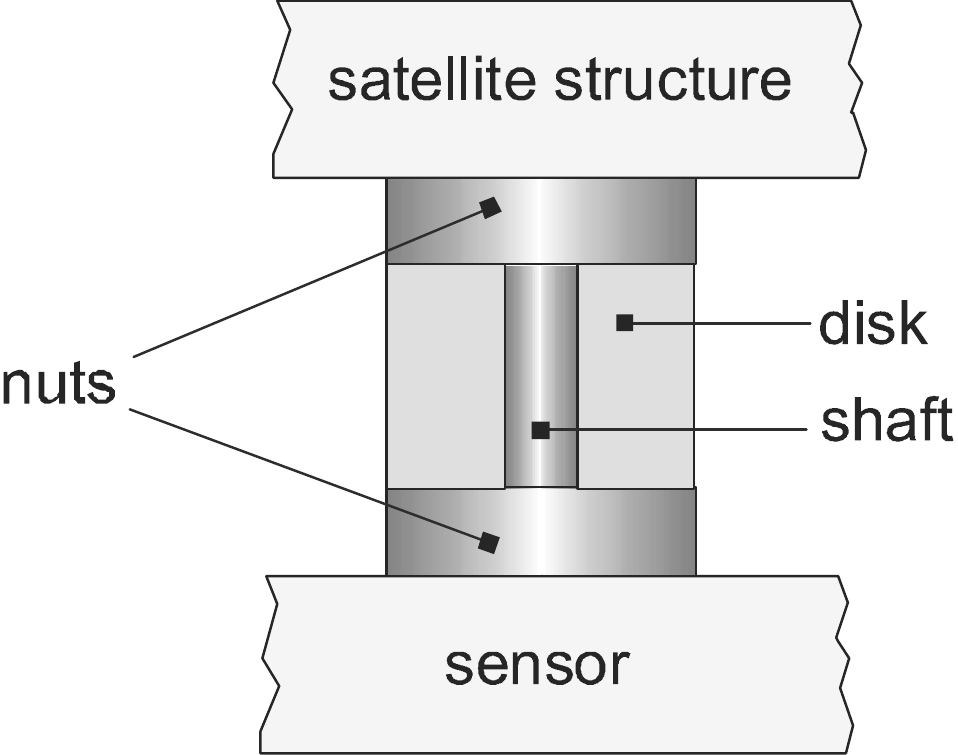
\includegraphics[height=0.18\textwidth]{Media/tcs_switch_01.png}\label{fig:tcs_switch11}}\qquad\qquad
	\subfloat[Open switch, reduced heat conduction.]{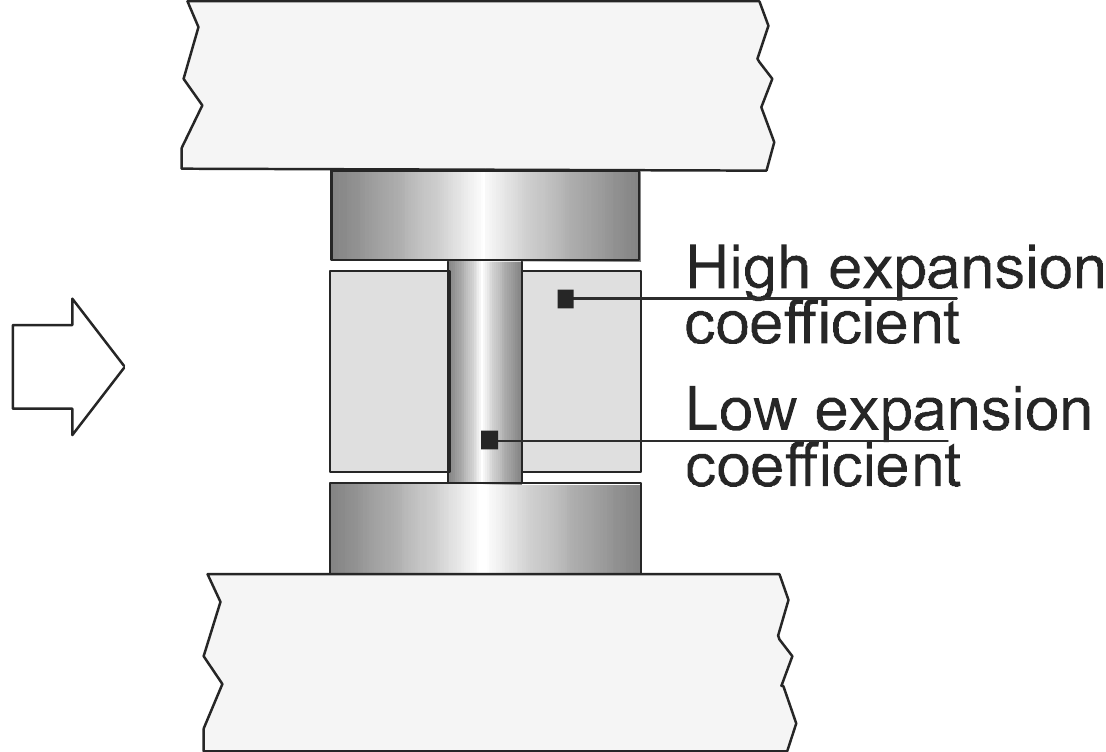
\includegraphics[height=0.18\textwidth]{Media/tcs_switch_02.png}\label{fig:tcs_switch12}}
	\caption{Bi-metallic heat switch, \cite{ref_tcs_04}.}
	\label{fig:tcs_switch01}
\end{figure}

\begin{figure}[H]
	\centering
	\subfloat[Comparison between data and theory (experimental results), \cite{ref_tcs_04} ]{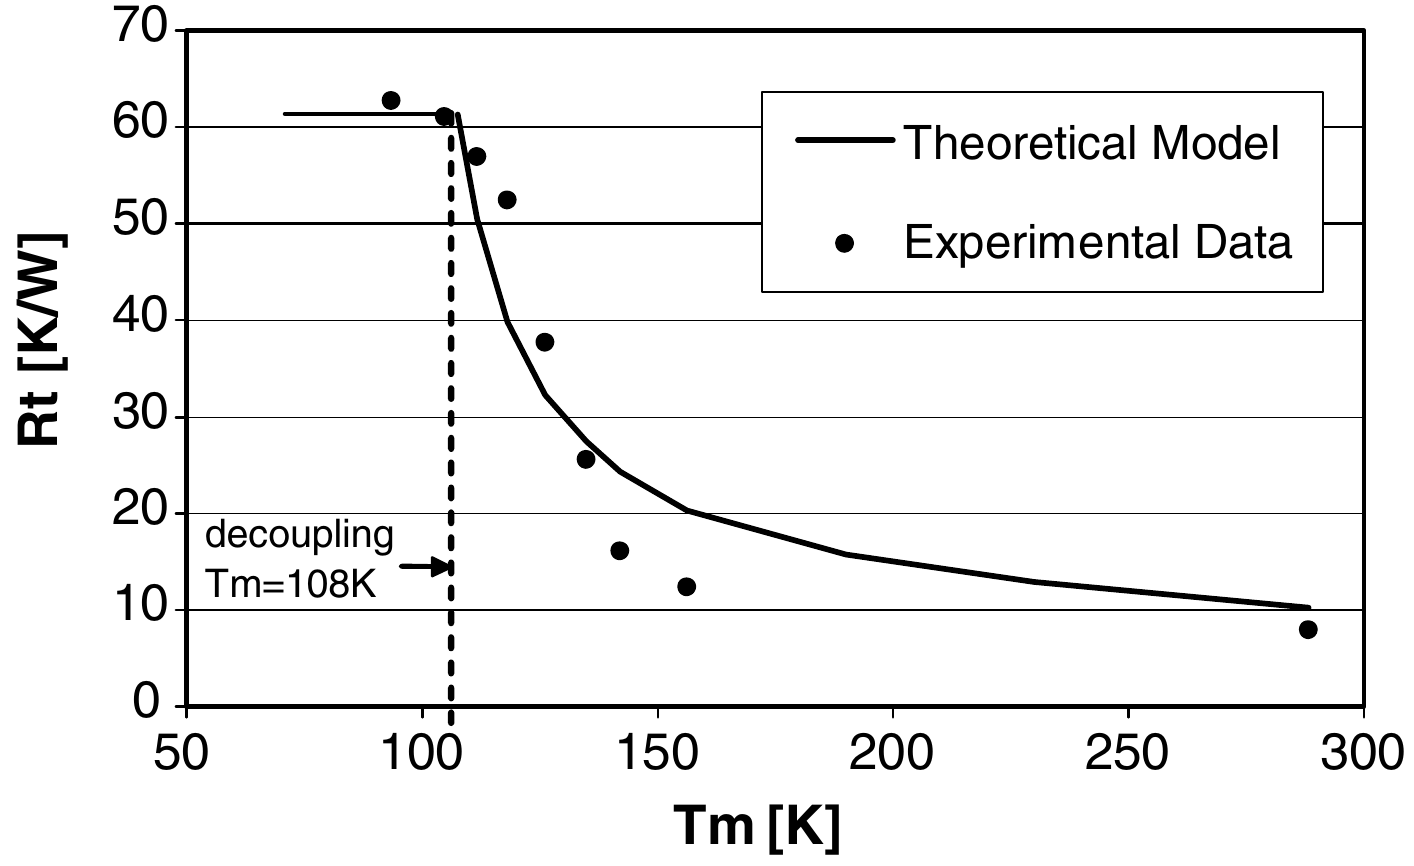
\includegraphics[height=0.22\textwidth]{Media/tcs_diag_orig.png}\label{fig:tcs_switch21}}\qquad
	\subfloat[Linearised characteristic of bi-metallic heat switch (red line).]{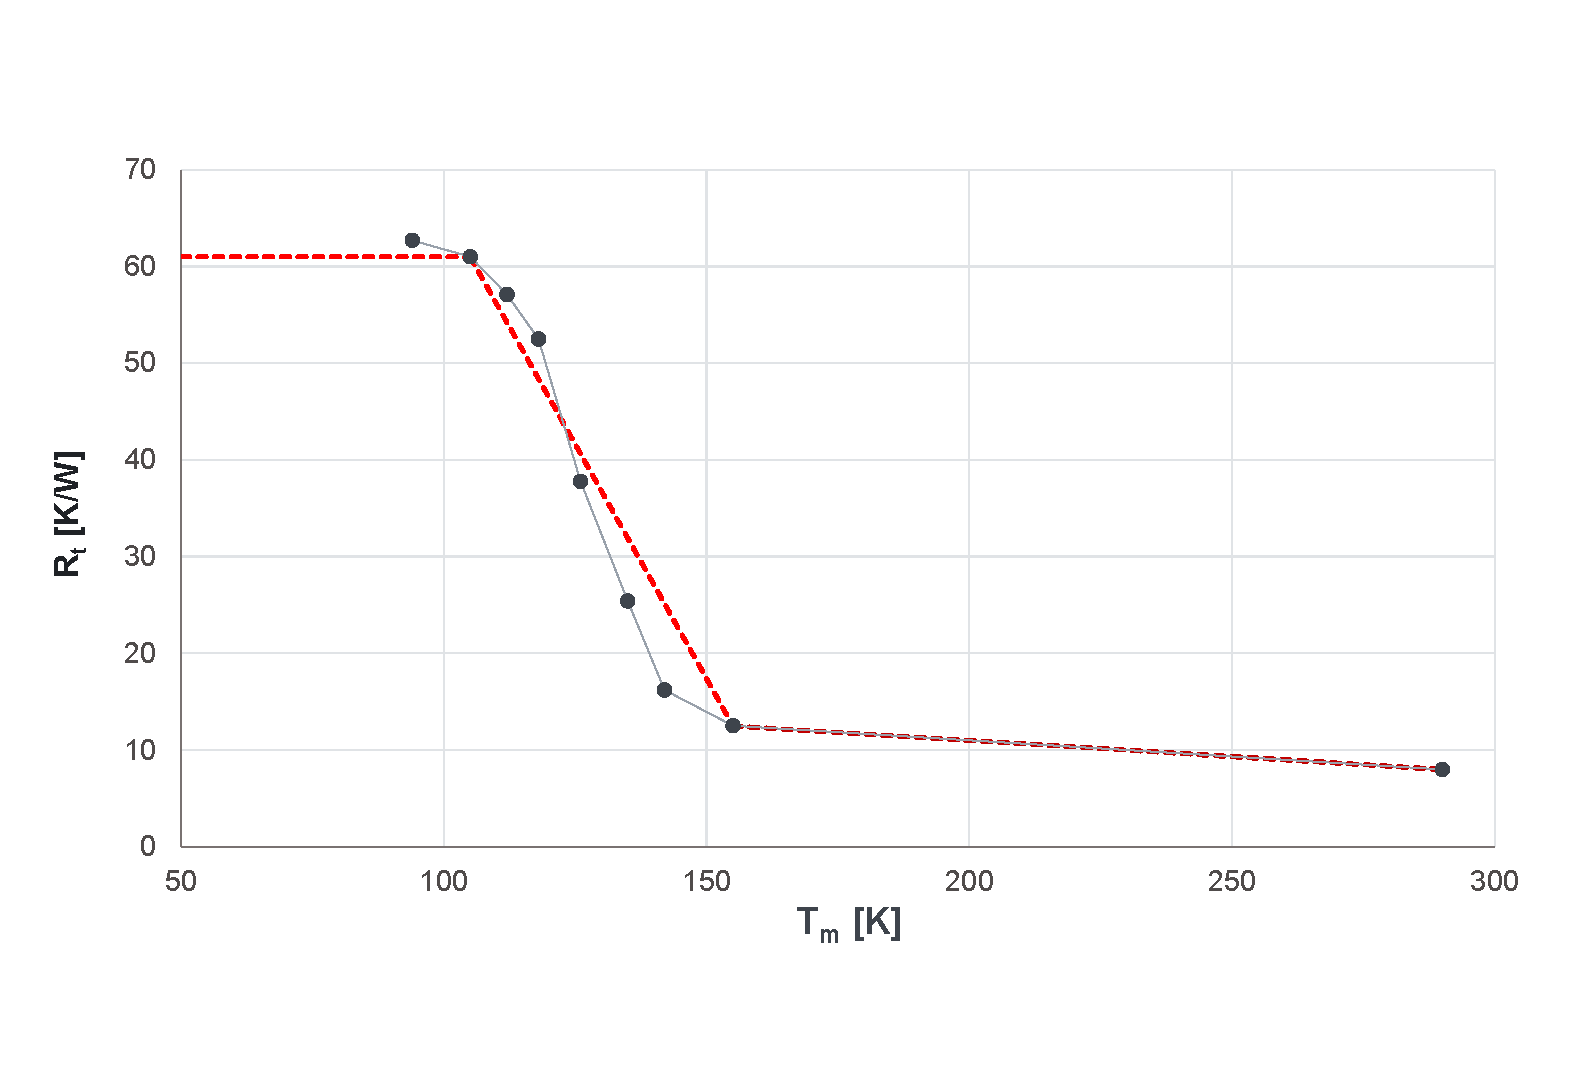
\includegraphics[height=0.22\textwidth]{Media/tcs_diag_lin}\label{fig:tcs_switch22}}
	\caption{Change of the heat switch conductivity $R_t$ over the mean temperature $T_M$.}
	\label{fig:tcs_switch02}
\end{figure}

\subsection{Thermal Network}
A thermal analysis was performed in order to get
\begin{itemize}
	\item the dimension of the insulation and heat straps,
	\item the necessary amount of RHUs and heat switches,
	\item the required surface finishing and
	\item the suitable choice of material.\\
\end{itemize}

For that, a thermal network with ten nodes was derived from the rover, shown in \autoref{fig:tcs_network}.
At the intersection of the steer and drive engine, two additional nodes were defined to calculate the heat flow.

\begin{figure}[h]
	\centering
	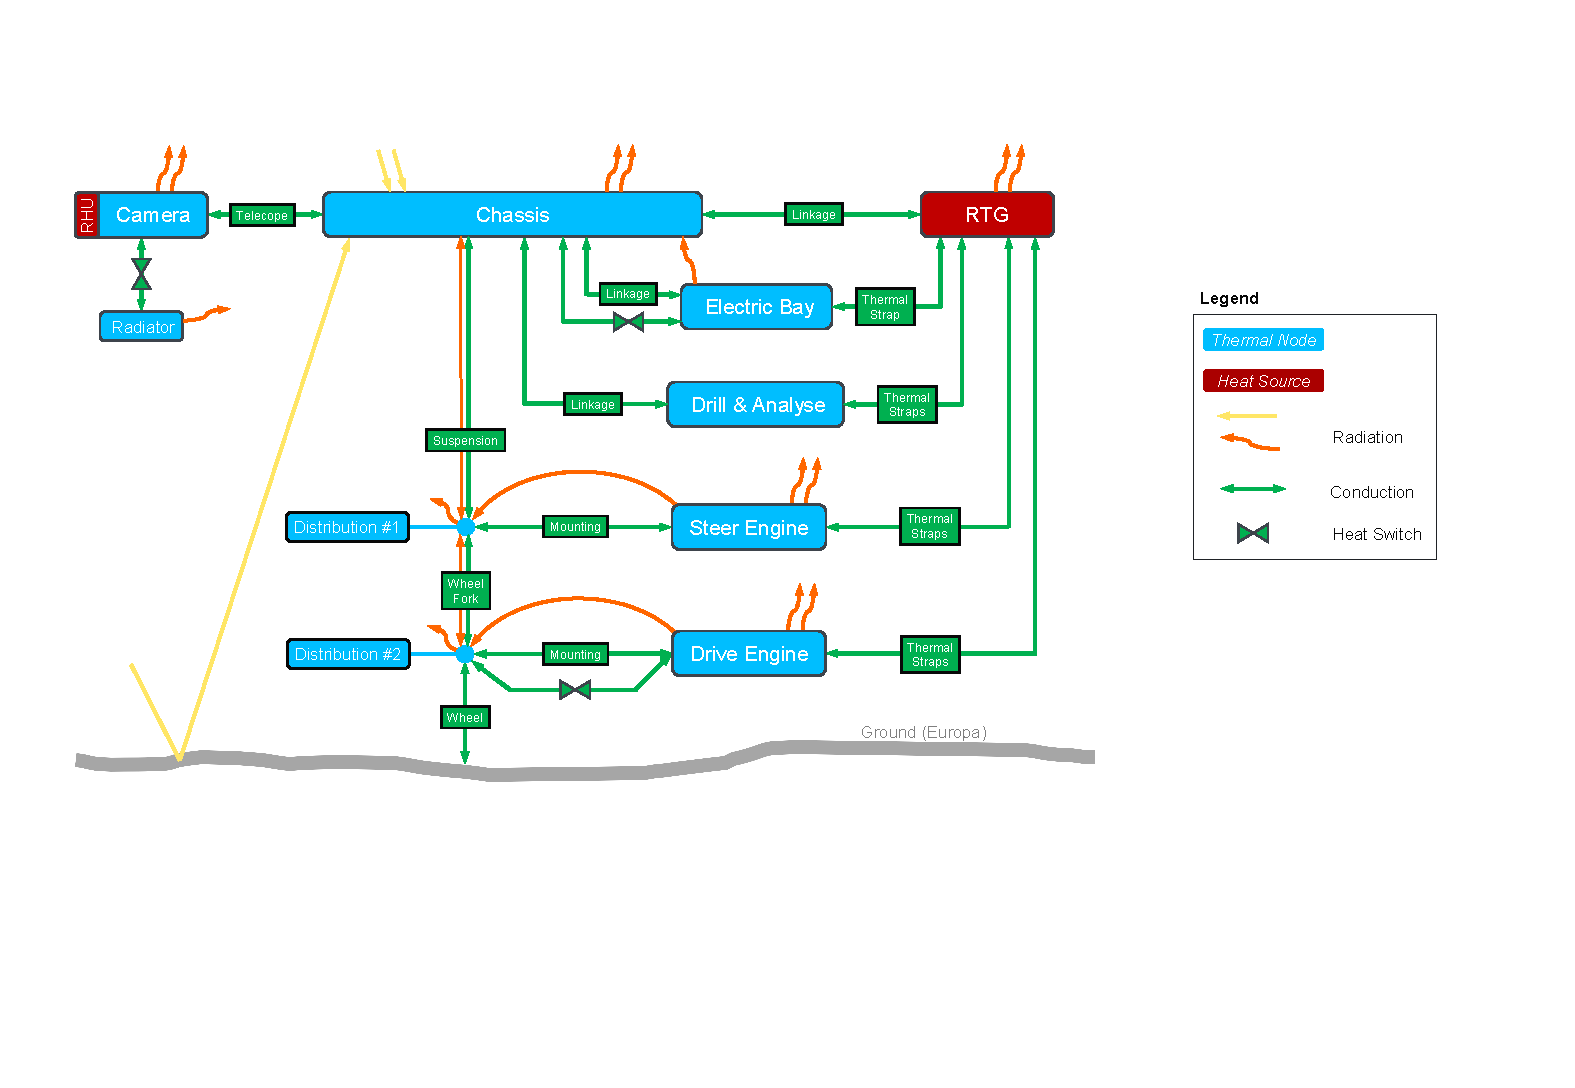
\includegraphics[width=0.85\textwidth]{Media/tcs_network}
	\caption{Thermal network of the rover.}
	\label{fig:tcs_network}
\end{figure}

On the basis of the thermal network, the heat energy equilibrium for each node was defined (see \appref{sec:app_tcs_01}).
The calculations were considered as a quasi-static analysis, where the component temperatures stay constant, $\frac{\dd T}{\dd t}=0$.
Following simplifications and assumptions for the analysis were made.
\begin{itemize}
	\item The convection was neglected due to the thin atmosphere.
	\item The whole electrical power of the components will be dissipated into heat.
	\item A variation of $\pm 20\%$ for the emissivity and absorptivity values was considered, if applicable (seet \autoref{tab:tcs_surface}).
	\item The heat as a result of retardation radiation inside the shielding was neglected.
	\item No discrete nodes for the radar, hazcams, APXS and deployment engines were considered. Their heat will be led into the chassis.
	\item The mechanism engines weren't considered.
	\item For the bogies  and the wheel fork radiation was defined. The radiation temperature is the mean temperature of the two connecting nodes. Half of the heat loss was added to corresponding nodes (either Chassis, Node$_1$ or Node$_2$).
\end{itemize}


\subsection{Analysis}
The thermal analysis was performed as an Excel calculation with the  possibility to adapt input values and dimensions, \autoref{app:DigitalAppendix} Nr. 1.
The major driving load cases are the  hot and the cold cases, where the maximum and minimum temperatures of the rover components will be reached.
For that, the most powerful components were set to operating mode at once or only the minimum required components were turned on, respectively.
The emissivity and absorptivity were adjusted to fulfil the cases.
There were further load cases defined to consider the  battery charging, the communication mode and the drill \& analyse operation.

\subsection{Results}
The resulting temperatures for each node over all loadcases  are listed in \autoref{tab:tcs_temp1}.
All temperatures lay between their limits without using a heater.
The margins for uncertainties, acceptance tests and qualification tests were considered with 5 K each, $\pm$15 K in total, \cite{ref_tcs_05}.
The corresponding temperatures are listed in \autoref{tab:tcs_temp2}.
Due to the margin, the electric ebay exceeds the temperature limits of the transmitter.
The issue can be solved by optimising the heat paths and adding further insulation during a detailed ebay design process.
Yet another result can be found in \autoref{tab:tcs_nodes1} to \autoref{tab:tcs_nodes5}, \autoref{tab:tcs_toggle} and  \autoref{tab:tcs_lynx}.


%-------------------------------------------------------------------------------
\section{Radiation} \label{sec:Radiation}
%-------------------------------------------------------------------------------

Compared to the radiation environment near Earth the radiation environment near Jupiter is multiple times stronger. It has the highest radiation levels of any planet in our solar systems \cite{JupiterRadiationEnvironment}. In order to survive these harsh environmental conditions, special emphasis must be placed on the radiation protection. In \autoref{fig:trappedprotonelectronfluxes}, the average trapped proton and electron fluxes on Europa's orbit around Jupiter are shown in comparison to the outer Van Allen radiation belt around Earth. However, in contrast to the Van Allen radiation belt, the duration within the radiation environment on Europa cannot be minimised and the rover has to be designed to withstand the entire mission duration of 30 days. \\ \\
In oder to design and evaluate different radiation protection approaches, different calculations have to be performed. For this purpose the ESA SPace ENVironment Information System (SPENVIS) is used \cite{Spenvis}. All calculations and figures in \autoref{sec:Radiation} are performed with SPENVIS unless otherwise stated.

\subsection{Radiation Protection}

\label{subsec:RadiationProtection}

Various options are available to protect the rover against the radiation. A common approach is the use of aluminium or titanium as these materials can also act as structural elements. However, due to the mass constraints of 30 kg other materials or material compositions are taken in consideration which are more mass effective. In \autoref{tab:OptimalRadiationProtection}, an optimised shield structure is presented for different weight thresholds designed for the radiation environment around Jupiter.

\begin{wraptable}{r}{8cm}
\centering
\caption{Optimal shield structure for an Jupiter mission. \cite{8823057}}
\begin{adjustbox}{max width=\textwidth}
\begin{tabular}[l]{cccccc}

	\toprule
	
	Areal Density	&	\(0.5\)	&	\(1\) &  \(2\) & \(3\)	\\
	/ \(\text{g/cm}^2\)	&	&	&  & \\
	
	\midrule
	
	
	Layer No. 1	&	Pb &  Pb & W	& Ta	\\
	/ mm	&	0.415 &  0.829 & 0.984	& 1.563	\\
	
	
	Layer No. 2	&	Fe	&  Mg &	Mg & Al \\
	/ mm	&	\(0.033\)	&  \(0.158\) &	\(0.540\) & \(0.399\) \\
	
	
	Layer No. 3 &	-	&  -	& - & Mg \\
	/ mm &	-	&  -	& - & \(0.150\) \\
	

	\bottomrule

\end{tabular}
\end{adjustbox}
\label{tab:OptimalRadiationProtection}
\end{wraptable}

The difference between an aluminium or titanium shielding and an optimised structure listed in \autoref{tab:OptimalRadiationProtection} for the total ionizing dose (TID) is shown in \autoref{fig:AluminiumTitanOptimised}. \\ \\
Due to the mass savings of the optimised structure it will be used where the radiation protection of the aluminium structure is not sufficient. In order to reduce the mass further, a radiation vault is utilised that highly sensible components do not have to be shielded separately.

\subsection{Components}

\label{subsec:RadiationComponents}

Every component on the rover has a different radiation tolerance and therefore have to be placed at different compartments within the rover. The radiation tolerances are listed in \autoref{tab:RadiationList}. None sensitive components like the electric motors and harness are only shielded by an aluminium structure where components like the metal within the wire are resistant against the radiation. However, isolators around the cables have to be selected to be resistant in order to prevent short circuits. Highly sensitive components like cameras have an additional protective layer in order to reduce the TID to under 30 krad. Components which are within the rover like the on-board computer (OBC) are placed within the radiation vault which reduces the TID to under 20 krad. For this purpose the optimised shield structure with a weight target of 0.5 \(\text{g/cm}^2\) is used. Detailed TIDs for all components are shown in \autoref{fig:CompartmentTID}.

\subsection{Improvements}

\label{subsec:RadiationImprovements}

Even though the radiation protection is sufficient for the rover to survive at least the nominal mission of 30 days, further improvements can be performed in order to extend the secondary mission. \\ \\
Local shielding can be applied on less resistant components in order to reduce the wall thickness of the whole radiation wall. If components with a radiation tolerance under 43.27 krad are individually shielded a mass saving of 736.2 g can be achieved. Additionally, water ice extracted from the surface of Europa can be used to improve the radiation protection. With a layer of one centimetre of water, the TID within the radiation vault can be reduced to 16.03 krad without the additional radiation protection beside the 4 mm of aluminium structure. The start mass of the rover can therefore be reduced by 897.2 g by removing the additional shielding. \\ \\
Detailed calculations for local shielding and water improvements can be found in \apprefsub{app:AppendixRadiationImprovements} and may be analysed further in Phase B.

\subsection{Conclusion}

\label{subsec:RadiationConclusion}

In order to protect the rover against the high radiation levels at the surface of Europa, the rover has different compartments. High sensible components are placed within a radiation vault which has a mass optimised structure. Components which has to be outside the radiation vault but are highly sensible are shielded individually. Low sensible Components are protected by the Aluminium structure. \autoref{fig:RadiationOverview} illustrates the different compartments within the rover and the accorded TIDs.

\begin{figure}[htb]
     \centering
     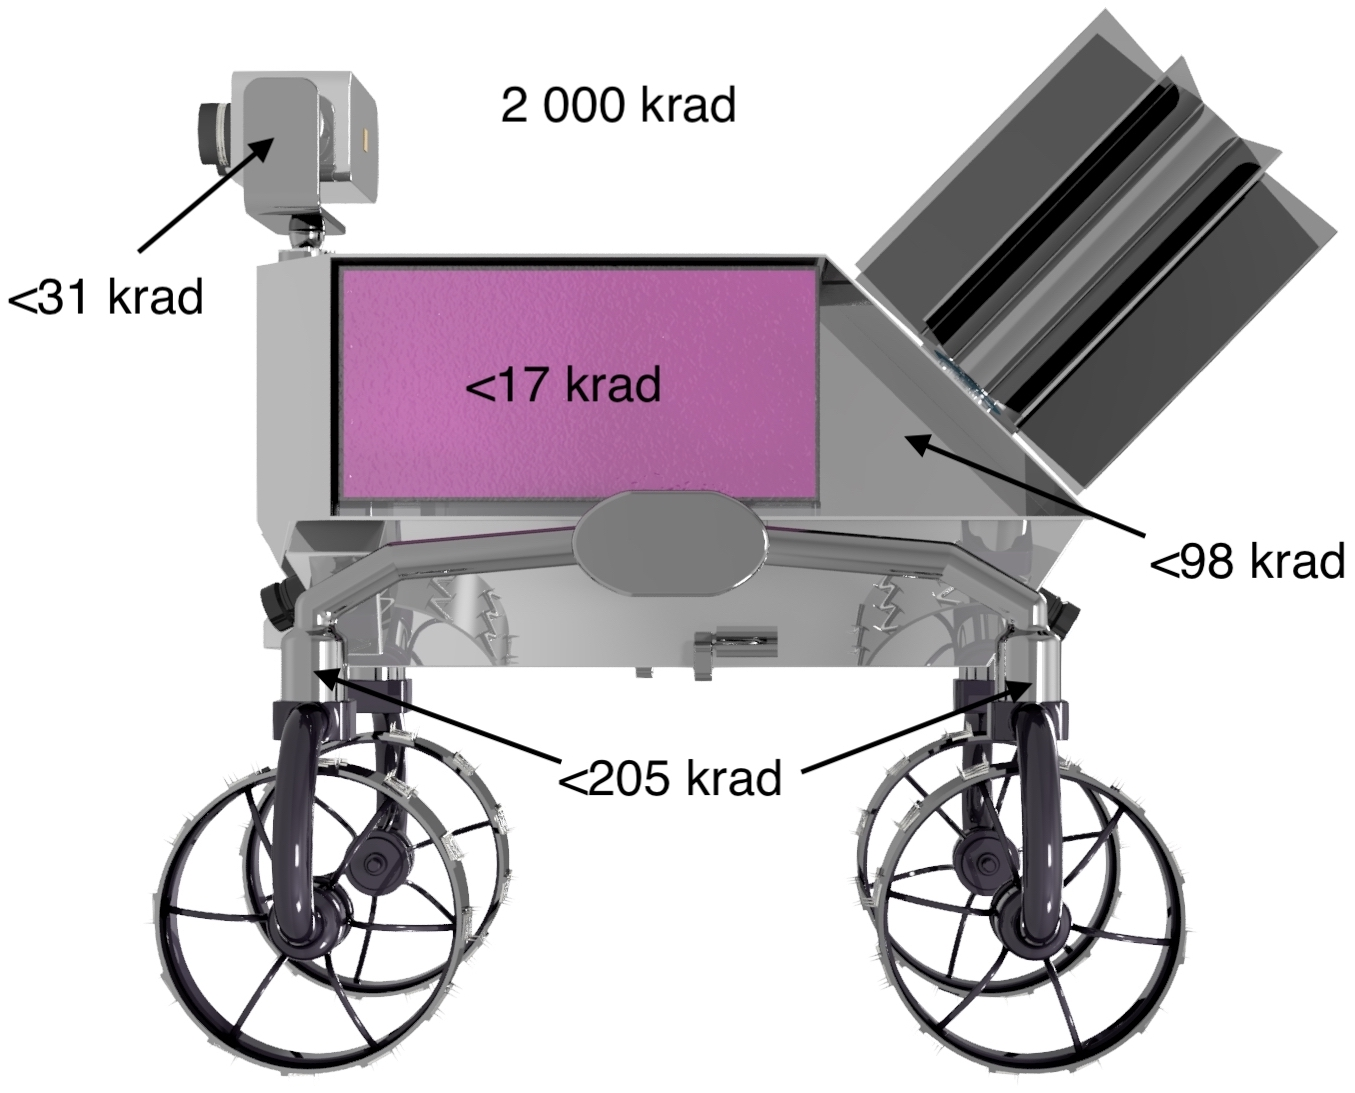
\includegraphics[width=\textwidth]{Media/INSPIRE_Radiation}
     \caption{Overview of TIDs within different compartments within the rover.}
     \label{fig:RadiationOverview}
\end{figure}

\clearpage